% The Berkeley admissions case as a causal graph, adapted from Chiappa (2019, Fig. 1): gender A
% affects admission directly (unfair, red) and through the choice of department X_1 (fair, so X_1
% is a resolving variable, shaded); X_2 is the applicant's qualifications.
% Compile on its own (pdflatex path-specific-graph.tex); the thesis includes the PDF.
% Same styles as scm-running-example.tex and same-distribution-graph-*.tex.
\documentclass[12pt,border=2pt]{standalone}
\usepackage[T1]{fontenc}
\usepackage{mathpazo}
\usepackage{tikz}
\usetikzlibrary{arrows.meta}
\begin{document}
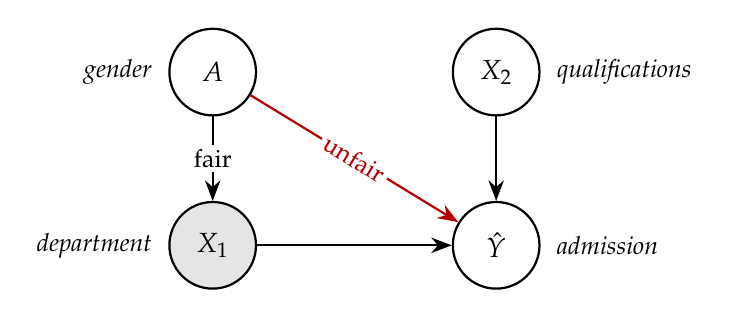
\begin{tikzpicture}[
    var/.style       = {circle, draw, thick, minimum size=11mm, inner sep=0pt},
    resolving/.style = {var, fill=gray!20},
    arr/.style       = {-{Stealth[length=2.6mm]}, thick},
    unfair/.style    = {arr, red!70!black},
    lab/.style       = {font=\small, fill=white, inner sep=1.5pt},
    word/.style      = {font=\small\itshape}
  ]
  \node[var]       (A)  at (0, 2.2)   {$A$};
  \node[var]       (X2) at (3.6, 2.2) {$X_2$};
  \node[resolving] (X1) at (0, 0)     {$X_1$};
  \node[var]       (Y)  at (3.6, 0)   {$\hat{Y}$};

  \draw[arr]    (A)  -- node[lab] {fair} (X1);
  \draw[unfair] (A)  -- node[lab, text=red!70!black, sloped] {unfair} (Y);
  \draw[arr]    (X2) -- (Y);
  \draw[arr]    (X1) -- (Y);

  \node[word, left=6.5mm]  at (A)  {gender};
  \node[word, right=6.5mm] at (X2) {qualifications};
  \node[word, left=6.5mm]  at (X1) {department};
  \node[word, right=6.5mm] at (Y)  {admission};
\end{tikzpicture}
\end{document}
